\section{Mediciones}

\subsection{Construcción de las entradas}

Para generar los archivos de entrada hicimos un script en lenguaje Python.

El primer bloque de código genera un archivo llamado ``medicionesConSpanVariable.in''. Se fijan primero las constantes \emph{h}, \emph{carga}, \emph{C} y \emph{fMax}
(Las dos últimas no serán utilizadas, se agregan por consistencia, la carga se usará para todas las juntas por igual y será fija, al igual que la altura). 
Luego se procede a ciclar el span entre un valor mínimo y uno máximo, aumentando en 1 su valor, lo mismo se hace para \emph{n}, en un ciclo interno. 
Como resultado el archivo tendrá varias instancias separadas por líneas en blanco, con el mismo formato que pide la cátedra, con altura y cargas fijas, y span y secciones variables.

El segundo bloque de código hace algo muy parecido, generando el archivo llamado ``medicionesConCargaVariable.in''. En vez de fijar \emph{carga} se fijará \emph{span}, y se
procederá a ciclar entre cargas mínimas y máximas.
Éste archivo tendrá varias instancias separadas por líneas en blanco, con altura y span fijo, y cargas y secciones variables.


\subsection{Resultados}

\subsubsection{Span Variable}

\begin{figure}[H]
  \centering
    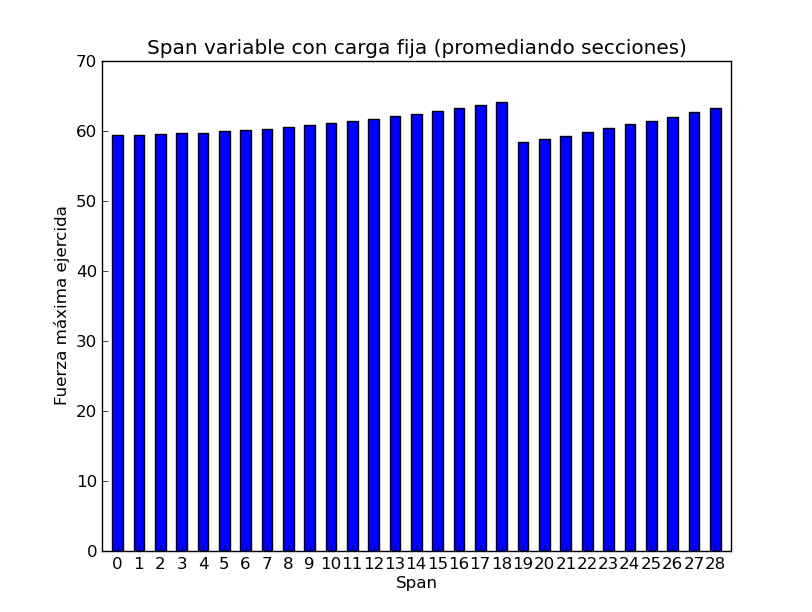
\includegraphics[width=0.9\textwidth]{../mediciones/spanVariable.png}
    \caption{}
\end{figure}

\'Este experimento se realiz\'o con una altura igual a 10, una carga igual a 25 (la misma en todas las juntas) y un span variando entre 1 y 30. 
Tambi\'en variamos para cada span la cantidad de secciones (n = 2, 4, 6, 8) y luego promediamos los resultados. 

Un resultado particular que encontramos fue que sin importar el valor del span, vimos que para n = 2, la fuerza m\'axima era mayor que las dem\'as
(las cuales crec\'ian ascendentemente para n mayor a 2); observando los dibujos de puentes, pensamos que puede deberse a que teniendo solamente 2 secciones,
habr\'ia un solo link (el del medio) sosteniendo toda la carga, al contrario de los puentes con 4 o m\'as secciones, las cuales se dividen dicha carga
entre por lo menos 2 links.

Dejando de lado el valor para cada n, tambi\'en vimos que a medida que aumentamos el span, la fuerza m\'axima de un link crece ``semi-ascendentemente'', aunque con
muy poco cambio, siendo casi despreciable, como se ve en el gr\'afico. Otra cosa particular que vimos fue que hay un punto (span = 19) donde la fuerza
m\'axima disminuye (por eso lo de ``semi-ascendente''), aunque luego continua con su crecimiento; pensamos que tal vez se debe a alg\'u cambio l\'imite 
en el \'angulo de los links.

 
\subsubsection{Carga Variable}

\begin{figure}[H]
  \centering
    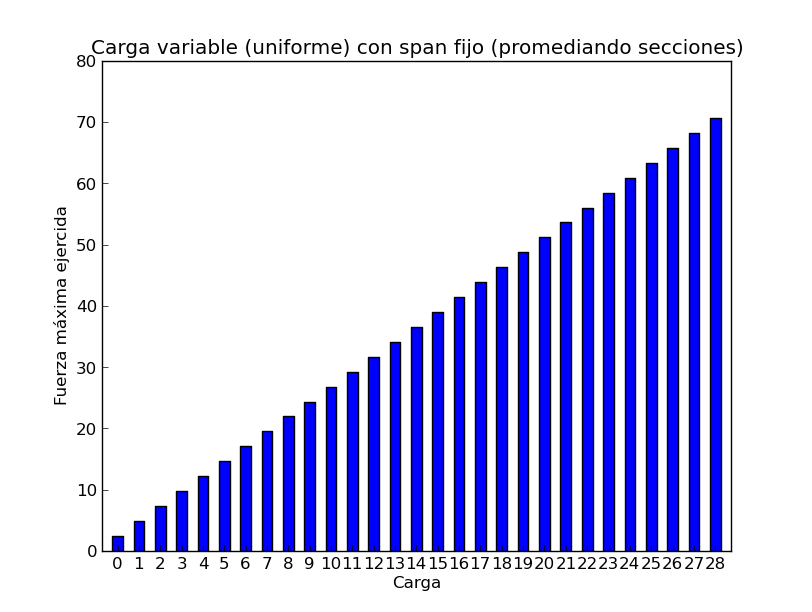
\includegraphics[width=0.9\textwidth]{../mediciones/cargaVariable.png}
    \caption{}
\end{figure}

\'Este experimento se realiz\'o con una altura igual a 10, un span igual a 25 y cargas variando entre 1 y 30 (la misma en todas las juntas). 
Tambi\'en variamos para cada carga la cantidad de secciones (n = 2, 4, 6, 8) y luego promediamos los resultados. 

El resultado fue un gr\'afico ascendente y completamente lineal en funci\'on de la carga, tal como esper\'abamos.
Al dejar fijo el span y la altura, los \'angulos no entran en juego, y obviamente la fuerza m\'axima solo depender\'a de la carga.